\section{Judas - Software Framework}

The DAS folder has not changed much substantially. The main difference from before is how we now instead of writing matrix data to one large binary file, data is split into multiple files, and only read when needed.

Contrary to what was mentioned before, the output of the function \texttt{load\_DAS\_files} has actually changed. Previously, we stored a whole vector of the timestamps for each sample. Not only was this cistly, but actaully totally redundant. If the timestamp of the first row is known, the sampling rate $T$ and which row to look at, one can instead calculate the timestamp like this: 
\lstinline|start_time + MilliSecond(idx * T * 1000)|. This in-place calculation can be done multiple times effectively in Julia using the broadcast operator (.). This ensures that we don't lose essential information before running our data through through the autoencoder

\begin{figure}[h]
\centering
\begin{subfigure}{.45\textwidth}
  \centering
  \lstinputlisting[language=Julia]{code/dasstructold.jl}
  \caption{Old DAS Struct}
  \label{fig:olddasstc}
\end{subfigure}%
\hfill
\begin{subfigure}{.45\textwidth}
  \centering
  \lstinputlisting[language=Julia]{code/dasstruct.jl}
  \caption{New Layout for DAS struct}
  \label{fig:newdasstc}
\end{subfigure}
\caption{Comparison between different versions of the DAS struct}
\label{fig:dasstccmp}
\end{figure}



\textbf{API Usage}

\begin{figure}[h]
    \centering
    \lstinputlisting[language=Julia]{code/apiusage.jl}
    \caption{How to use our API}
    \label{fig:apiusage}
\end{figure}


\begin{figure}[h]
    \centering
    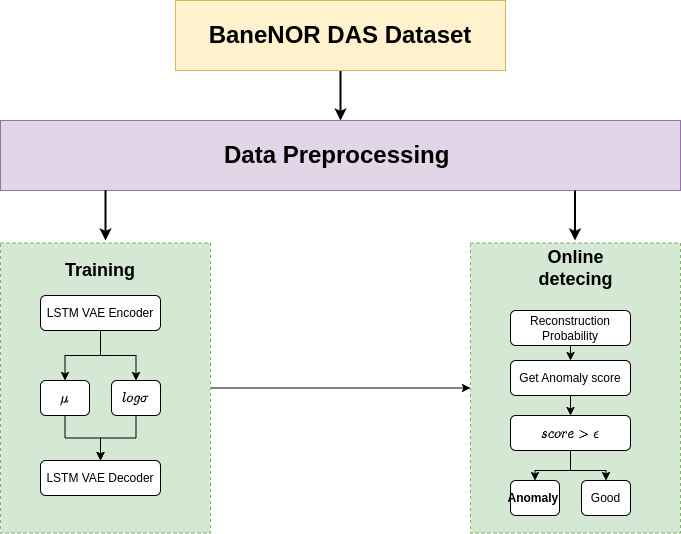
\includegraphics[scale=0.5]{figures/methodflow.png}
    \caption{Dataflow}
    \label{fig:dataflow}
\end{figure}


